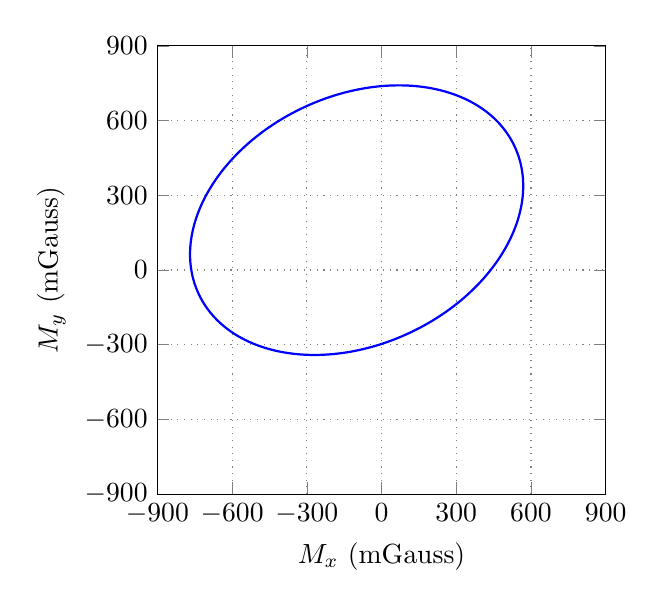
\begin{tikzpicture}
        \begin{axis}[
            axis equal image,
            grid=both,
            grid style={dotted, gray},
            xmin=-900, xmax=900,
            ymin=-900, ymax=900,
            xlabel={$M_x$ (mGauss)},
            ylabel={$M_y$ (mGauss)},
            xtick={-900,-600,-300,0,300,600,900},
            ytick={-900,-600,-300,0,300,600,900},
        ]

         % Plot the ellipse with correct offset and rotation
        \draw[blue, thick, rotate around={25:(axis cs:-100,200)}] (axis cs:-100,200) ellipse [x radius=700, y radius=500];
    \end{axis}
\end{tikzpicture}